\section*{Übung 10}
\subsection*{Aufgabe 1}
\subsubsection*{Lösungsidee}
Es wird eine Prozedur erstellt, basierend auf der vorgeschlagenen Lösungsidee. Um die Größe des Arrays festlegen zu können wird die Anzahl der Nodes im Baum mithilfe von CountNodes ermittelt. Nachdem das Array initialisiert wurde und alle Nodes des Baumes in das Array eingefügt sind, werden die Mittelpositionen berechnet. Mit den berechneten Werten wird bestimmt welche Elemente des Arrays eingefügt werden. Elemente die bereits in den Baum gespeichert wurden, werden im Array auf NIL gesetzt. Alle fehlenden Elemente werden danach eingefügt.
\newline

\lstinputlisting[language=Pascal] {../balancedtree.pas}
\begin{figure}[H]
	\centering
	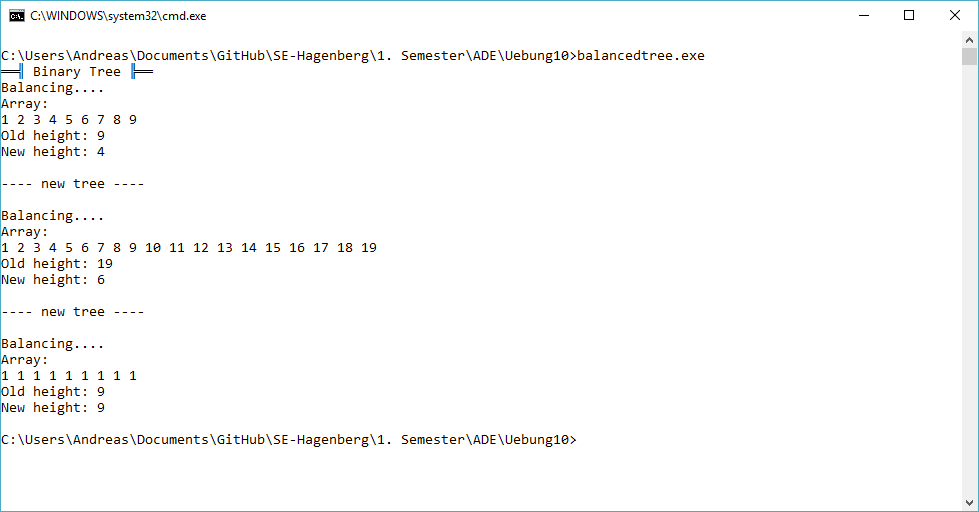
\includegraphics[scale=0.65]{./pictures/balancedtree.png}
	\caption{Testfälle}
	\label{fig: BalancedTree}
\end{figure}

\subsection*{Testfälle}
Die Testfälle zeigen drei verschiedene Bäume mit unterschiedlicher Länge und Werten. Anhand des dritten Baumes wird ersichtlich das bei gleichen Werten die Höhe des Baumes nach dem Balancieren die gleiche ist wie davor.

\subsection*{Zusatzfrage}
Da bei diesem Baum nicht extra spezifiziert wurde was mit gleichen Werten geschehen soll wird immer nur in eine Richtung eingefügt, die Zahl ist schließlich nicht größer als die Wurzel oder der jeweilige Knoten. Damit ergibt sich selbst nach dem ausführen des Algorithmus immer noch dieselbe Höhe.
\newpage




